\documentclass[11pt,handout,aspectratio=169,dvipsnames]{beamer}

\usepackage{listings}
\lstset{
    language=R,                     % Specify R as the programming language
    basicstyle=\ttfamily\scriptsize,      % Set font to typewriter (\ttfamily) and small size
    keywordstyle=\color{blue},       % Color for R keywords
    commentstyle=\color{gray},       % Color for comments
    stringstyle=\color{red},         % Color for strings
    numbers=left,                    % Line numbers on the left
    numberstyle=\tiny\color{gray},   % Small gray line numbers
    stepnumber=1,                     % Number every line
    breaklines=true,                 % Line breaking enabled
%    frame=single,                    % Single-line frame around code
    captionpos=b,                     % Caption position at bottom
    tabsize=2                         % Set tab size to 2 spaces
}
\usepackage{multirow}

%%%%%%%%% GENERAL PACKAGES
%\usepackage{xcolor}
%\usepackage{pdfpages}
%\usetheme[progressbar=frametitle]{metropolis}
%\setbeamercolor{background canvas}{bg=white}
%\usepackage{appendixnumberbeamer}
%\usepackage{booktabs}
%\usepackage[scale=2]{ccicons}
%\usepackage{pgfplots}
%\usepgfplotslibrary{dateplot}
%\usepackage{xspace}
%\newcommand{\themename}{\textbf{\textsc{metropolis}}\xspace}
%\usepackage[absolute,overlay]{textpos}

%%%%%%%%% COLOR THEME

% Define some colors:
\definecolor{DarkFern}{HTML}{407428}
\definecolor{DarkCharcoal}{HTML}{4D4944}
\definecolor{AlertColor}{RGB}{89,124,158}
\definecolor{HighLight}{RGB}{96,95,134}
\definecolor{Important}{RGB}{234,122,133}
\definecolor{Yellow}{HTML}{00539C}
\colorlet{Fern}{DarkFern!85!white}
\colorlet{Charcoal}{DarkCharcoal!85!white}
\colorlet{LightCharcoal}{Charcoal!50!white}
\colorlet{HighLight2}{AlertColor}
\colorlet{DarkRed}{red!70!black}
\colorlet{DarkBlue}{blue!70!black}
\colorlet{DarkGreen}{green!70!black}
\definecolor{RoyalBlue}{HTML}{00539C}
\definecolor{Peach}{HTML}{EEA47F}
\definecolor{ForestGreen}{HTML}{2C5F2D}
\definecolor{MossGreen}{HTML}{E8FCC9}
% Use the colors:
\setbeamercolor{title}{fg=Fern}
\setbeamercolor{frametitle}{fg=MossGreen,bg=ForestGreen}
\setbeamercolor{normal text}{fg=Charcoal!70!black}
\setbeamercolor{block title}{fg=black,bg=Fern!25!white}
\setbeamercolor{block body}{fg=black,bg=Fern!10!white}
\setbeamercolor{block title alerted}{fg=black,bg=DarkRed!25!white}
\setbeamercolor{block body alerted}{fg=black,bg=DarkRed!10!white}
\setbeamercolor{alerted text}{fg=DarkRed}
\setbeamercolor{itemize item}{fg=Charcoal}



%%%%%%%%% OTHER COMMANDS
\newcommand{\indep}{\perp\!\!\! \perp}
\newcommand{\comment}[1]{}
\newcommand{\bs}{\boldsymbol}
\newcommand{\tr}{\text{trace}}
\newcommand{\sgn}{{\rm sgn}}
\def\T{\top}
%\newcommand{\det}{\text{det}}
\newcommand{\var}{\mathrm{var}}
\newcommand{\cC}{{\cal C}}
\newcommand{\cG}{{\cal G}}
\newcommand{\cV}{{\cal V}}
\newcommand{\cE}{{\cal E}}
\newcommand{\cM}{{\cal M}}
\newcommand{\cP}{{\cal P}}
\newcommand{\cX}{{\cal X}}
\newcommand{\cY}{{\cal Y}}
\newcommand{\X}{\mathbf{X}}
\newcommand{\Y}{\mathbf{Y}}
\newcommand{\x}{\mathbf{x}}
\newcommand{\y}{\mathbf{y}}
\newcommand{\z}{\mathbf{z}}

\newcommand{\argmin}{\operatornamewithlimits{argmin}}
\newcommand{\eps}{\varepsilon}
\newcommand{\<}{\langle}
\renewcommand{\>}{\rangle}


\setbeamertemplate{itemize subitem}{\tiny\raise1.5pt\hbox{\donotcoloroutermaths$\blacktriangleright$}}
\setbeamertemplate{itemize subsubitem}{\tiny\raise1.5pt\hbox{\donotcoloroutermaths$\blacktriangleright$}}
\setbeamertemplate{enumerate item}{\insertenumlabel.}
\setbeamertemplate{enumerate subitem}{\insertenumlabel.\insertsubenumlabel}
\setbeamertemplate{enumerate subsubitem}{\insertenumlabel.\insertsubenumlabel.\insertsubsubenumlabel}
\setbeamertemplate{enumerate mini template}{\insertenumlabel}

\newcommand{\TODO}[1]{{\color{red}{[TODO: #1]}}}


\newcommand{\R}{\mathbb R}
\newcommand{\E}{\mathbb E}
\renewcommand{\P}{\mathbb P}


\DeclareMathOperator*{\cov}{cov}


\newsavebox{\zerobox}
\newenvironment{nospace}
{\par\edef\theprevdepth{\the\prevdepth}\nointerlineskip
  \setbox\zerobox=\vtop to 0pt\bgroup
  \hrule height0pt\kern\dimexpr\baselineskip-\topskip\relax
}
{\par\vss\egroup\ht\zerobox=0pt \wd\zerobox=0pt \dp\zerobox=0pt
  \box\zerobox}

\usepackage{soul}
\makeatletter
\let\HL\hl
\renewcommand\hl{%
  \let\set@color\beamerorig@set@color
  \let\reset@color\beamerorig@reset@color
  \HL}
  \makeatother


\title[STA437-Week1]{STA 437/2005: \\ Methods for Multivariate Data}
\subtitle[]{Week 11: Conditional independence}
\author[Piotr Zwiernik]{Piotr Zwiernik}
\institute[UofT]{University of Toronto}
\date{}


%\usepackage{Sweave}

\begin{document}

\maketitle

\begin{frame}[plain,noframenumbering]{}
\begin{center}
	{\huge \textcolor{DarkRed}{Basic definitions}}
\end{center}
\end{frame}

\begin{frame}{Random vector and independence}
	Let $(X,Y)$ be a vector of two random variables.
	\begin{alertblock}{Joint distribution}
		\textcolor{SeaGreen}{Density function} $f_{XY}(x,y)$ if continuous.\\[.1cm]
		\textcolor{SeaGreen}{Probability mass function} $f_{XY}(x,y)=\P(X=x,Y=y)$ if discrete.
	\end{alertblock}
		\begin{alertblock}{Marginal distribution}
continuous:\;\;\;$f_X(x)=\int_\R f_{XY}(x,y){\rm d}y$.\\[.1cm]
discrete:\;\;\;$f_X(x)=\sum_y f_{XY}(x,y)=\P(X=x)$.
	\end{alertblock}
	This can be generalized to random vectors.
\end{frame}

\begin{frame}{Independence}
\begin{beamercolorbox}[wd=\paperwidth,sep=2pt]{goldbox}
	If $f_{XY}(x,y)$ is the joint density (or PMF) of $(X,Y)$ then $X$ and $Y$ are independent if and only if \\[-.5cm] $$ f_{XY}(x,y)=f_X(x)f_Y(y)\qquad\mbox{for all }x,y.$$
		We write \alert{$X\indep Y$}.	
\end{beamercolorbox}
		Recall:
		$$
		\cov(X,Y)=\E(XY)-\E(X)\E(Y)\quad\mbox{and}\quad \var(X)=\cov(X,X).
		$$
		The correlation $\rho_{X,Y}$ between $X,Y$ is:
		$$
		\rho_{X,Y}\;=\;\tfrac{\cov(X,Y)}{\sqrt{\var(X)\var(Y)}}\;\in\;[-1,1].
		$$
		\begin{beamercolorbox}[wd=\paperwidth,sep=2pt]{important}
			If $X\indep Y$ then $\rho_{X,Y}=0$.\\ {\footnotesize(but in general not the other way around, see slide \ref{zerocor})}
		\end{beamercolorbox}
\end{frame}

\begin{frame}{Conditional distribution}
	\begin{block}{Conditional distribution}
		In the discrete case the conditional probability mass function is defined as
		$$f_{X|Y}(x|y)=\textcolor{DarkRed}{\P(X=x|Y=y)}=\tfrac{\P(X=x,Y=y)}{\P(Y=y)}  $$ 
		for all  $x,y$ such that  $\P(Y=y)>0$ and so $$f_{X|Y}(x|y)=\tfrac{f_{XY}(x,y)}{f_Y(y)} \mbox{ for all } x,y \mbox{ s.t. }f_Y(y)>0. $$ \textbf{In the continuous	case we use the same definition.}\end{block}
		\begin{alertblock}{Important reformulation of independence}
			$X\indep Y$ if and only if $f_{X|Y}(x|y)=f_X(x)$.\\
			(knowing $Y$ brings no extra information about $X$)
		\end{alertblock}

\end{frame}


\begin{frame}{A cautionary note}

	\begin{beamercolorbox}[wd=\paperwidth,sep=2pt]{notabene}	
Note: $f_{X|Y}(x|y)\neq f_{Y|X}(y|x)$.\\[.3cm] Example: A medical test for a disease $D$ has outcomes + and - with probabilities\\ 
{\centering\begin{tabular}{l|ll}
  & $D$  & $D^c$ \\ \hline
+ & .009 & .099  \\
- & .001 & .891 
\end{tabular}\\}
\bigskip

As needed $\P(+|D)=0.9$ and $\P(-|D^c)= 0.9$. However, $\P(D|+)\approx 0.08$ (!)
 \end{beamercolorbox}
\end{frame}

%
%
%\begin{frame}{Appendix: Conditional expectation}
%Let $X,Y$ have joint distribution $f_{XY}(x,y)$ and conditional $f_{X|Y}(x|y)$. Then the \textcolor{SeaGreen}{conditional expectation} $\E[X|Y]$ is the expectation of $X$ with respect to the conditional distribution $X|Y=y$.
%$$
%\E[X|Y=y]\;\;=\;\;\begin{cases}
%	\sum_x x \,f_{X|Y}(x|y)\\
%	\int_\R x \,f_{X|Y}(x|y){\rm d}x
%\end{cases}.
%$$ 
%It is clear that $\E[g(Y)X|Y]=g(Y)\E[X|Y]$.\\[.2cm]
%\textbf{Note that $\E[X|Y]$ is a function of $Y$ and so a random variable!}\\[.2cm]
%A powerful result states that $$\E\big[\E(X|Y)\big]\;=\;\E(X).$$ 	
%\vspace{-.4cm}\begin{alertblock}{Example: two binary variables}
%	Suppose $f_{XY}(0,0)=0.4$, $f_{XY}(0,1)=0.2$, $f_{XY}(1,0)=0.1$, $f_{XY}(1,1)=0.3$. Then\ldots
%\end{alertblock}
%\end{frame}
%


\begin{frame}{Conditional independence}
	$X,Y,Z$ random variables.\\[.3cm]
	\alert{$X$ is independent of $Y$ given $Z$} (write \textcolor{SeaGreen}{$X\indep Y|Z$}) if
	$$
	f_{XY|Z}(x,y|z)\;=\;f_{X|Z}(x|z)f_{Y|Z}(y|z)\qquad\mbox{for every }z.
	$$
%	We can define conditional expectation $\E(X|Z)$ and \alert{conditional correlation} :$$
%	\rho_{X,Y| Z}\;:=\;\tfrac{\cov(X,Y|Z)}{\sqrt{\var(X|Z)\var(Y|Z)}}
%	$$
%	\textbf{Note that these are functions of $Z$!}\\[.3cm]
%	
%	If $X\indep Y|Z$ \quad then\quad  $\rho_{X,Y| Z}\equiv 0$\\
%	\footnotesize{(but not the other way around)}
		\begin{alertblock}{Important reformulation of independence}
			$X\indep Y|Z$ if and only if $f_{X|Y,Z}(x|y,z)=f_{X|Z}(x|z)$.\\
			(if we observed $Z$, extra information about $Y$ brings no extra information about $X$)
		\end{alertblock}
\end{frame}

%\begin{frame}{Partial correlation}
%In practice we often work with the partial correlation:
%	$$
%	\rho_{X,Y\cdot Z}\;:=\;\tfrac{\rho_{X,Y}-\rho_{X,Z}\rho_{X,Y}}{\sqrt{(1-\rho_{X,Z}^2)(1-\rho_{Y,Z}^2)}}.
%	$$
%	We have $\rho_{X,Y\cdot Z}=0$ if and only if in the \textbf{linear} regression of $X$ on $Y,Z$ the coefficient of $Y$ is zero.
%	\begin{beamercolorbox}[wd=\paperwidth,sep=5pt]{important}	
%		We have $\rho_{X,Y\cdot Z}=\rho_{X,Y|Z}$ in the case of \textcolor{SeaGreen}{Gaussian}, elliptical, multinomial and Dirichlet distributions. But not in general.
%	\end{beamercolorbox}
%
%	\textbf{Important}: If  $\bs X=(X_1,\ldots,X_m)$ is a random vector with covariance matrix $\Sigma$, denote $K=\Sigma^{-1}$, then for each $i,j\in \{1,\ldots,m\}$ 
%	$$
%	\rho_{X_i,X_j\cdot X_{\{1,\ldots,m\}\setminus \{i,j\}}}\;=\;-\tfrac{K_{ij}}{\sqrt{K_{ii}K_{jj}}}.
%	$$ 
%	So normalizing the \textbf{concentration matrix} gives the partial correlations.
%	\begin{itemize}
%		\item $\rho_{X_i,X_j\cdot X_{\{1,\ldots,m\}\setminus \{i,j\}}}=0$ \quad$\Longleftrightarrow$\quad $K_{ij}=0$
%		\item $\rho_{X_i,X_j\cdot X_{\{1,\ldots,m\}\setminus \{i,j\}}}\geq 0$ \quad$\Longleftrightarrow$\quad $K_{ij}\leq 0$
%	\end{itemize} 
%\end{frame}


\subsection{Testing independence}
\begin{frame}[plain,noframenumbering]{}
\begin{center}
	{\huge \textcolor{DarkRed}{Testing independence}}
\end{center}
\end{frame}

\begin{frame}{Recall: A statistical test}
	Given a statistical hypothesis $H_0:$ $\theta\in \Theta_0$, $H_1:$ $\theta\in \Theta_1$, a statistical test consists of a \textcolor{SeaGreen}{test statistics} $T(X^{(1)},\ldots,X^{(n)})$ and a \textcolor{SeaGreen}{rejection region}, typically of the form
	$$
	R\;=\;\{T(X^{(1)},\ldots,X^{(n)})>t\}.
	$$ 
\begin{beamercolorbox}[wd=\paperwidth,sep=2pt]{notabene}	
If the null hypothesis is true $T$ is unlikely to take large values. \end{beamercolorbox}
\begin{alertblock}{Type I error:\quad $\P(T\in R|H_0)$} 
	although $H_0$ is true, it is rejected 
\end{alertblock}
\begin{alertblock}{Type II error:\quad $\P(T\notin R|H_1)$} 
	although $H_0$ is false, it is retained\end{alertblock}
\noindent A good test should minimize probabilities of both types of errors.\\[.2cm]
%\begin{beamercolorbox}[wd=\paperwidth,sep=2pt]{important}	
%The idea is that $T$ has some known distribution under $H_0$ so that we can compute the probability of $T\in R$ easily. \end{beamercolorbox}
\end{frame}

%\begin{frame}{Some vocabulary}
%\textcolor{SeaGreen}{Power function}: \quad $\beta(\theta)=\P_\theta(T(X_1,\ldots,X_n)\in R )$\\[.4cm]
%\textcolor{SeaGreen}{Size of a test}: \quad $\sup_{\theta\in \Theta_0}\beta(\theta)$ (want this small to minimize type I error)\\[.4cm]
%A test has \textcolor{SeaGreen}{level $\alpha$} if size is $\leq \alpha$.\\[.4cm]
%%\textcolor{SeaGreen}{Uniformly most powerful test}: (uniformly) highest power under $H_1$ among all size $\alpha$ tests, that is $\beta(\theta)\geq\beta'(\theta)$ for all $\theta\in \Theta_1$ and all tests $\beta'$.\\[.4cm]
%%\textcolor{SeaGreen}{Simple hypothesis}: \quad $H_0$: $\theta=\theta_0$, $H_1$: $\theta\neq \theta_0$.\\[.4cm]
%\end{frame}

%\begin{frame}[label={exgauss}]{Example: Zero mean in the Gaussian distribution}
%Let $X_1,\ldots,X_n$ be a sample from $N(\mu,1)$. We test $H_0$: $\mu=0$ versus $H_1$: $\mu\neq 0$ (simple hypothesis)\\[.4cm]
%Intuitively, if $|\bar X_n|$ is ``large'', we should reject $H_0$. Note that under $H_0$ we have $\sqrt{n}\bar X_n\sim N(0,1)$.\\[.4cm]
%The idea is to propose a test statistic with a known distribution (under $H_0$) so that computations are easy. In our case let: $$T(X_1,\ldots,X_n)\;=\; \left|\sqrt{n}\bar X_n\right|.$$
%We get a $\alpha$ level test when $t=z_{\alpha/2}$.\\[.2cm] For example, for $\alpha=0.05$ and $\alpha'=0.01$ we get \texttt{qnorm(1-0.05/2)}=1.96 and \texttt{qnorm(1-0.01/2)}=2.58. 
%\end{frame}

%\begin{frame}{$p$-value}
%	If $\alpha'<\alpha$ then a level $\alpha'$ test has ``smaller'' rejection regions than a level $\alpha$ test. If we reject at level $\alpha$ then we also reject at level $\alpha'$.\\[.2cm]
%	$\bullet$ The level $\alpha'$ test is more \textcolor{SeaGreen}{conservative}.\\[.4cm]
%	For a given data there exists a smallest $\alpha$ that leads to rejection. This $\alpha$ is called the \textcolor{SeaGreen}{p-value}.\\[.2cm]
%	$\bullet$ In the example on slide~\ref{exgauss}, suppose we observed $T=2.1$. Then the p-value is:\;\; 2(1-\texttt{pnorm}(2.1))=0.036.\\[.2cm]
%	$\bullet$ p-value is the same as the probability of the test statistic being greater than its observed value. We want this probability to be small. By convention smaller than $0.05$ is significant.\\[.4cm] 
%	\begin{beamercolorbox}[wd=\paperwidth,sep=3pt]{important}	
%Note: The p-value is not the probability that the null hypothesis is true, or the probability that the alternative hypothesis is false.
% \end{beamercolorbox}
%\end{frame}


\begin{frame}{Testing independence}
Data: $(X_1,Y_1)$, \ldots, $(X_n,Y_n)\overset{iid}{\sim}P_{X,Y}$.\\[.3cm]
Goal: Decide whether $X\indep Y$.\\[.3cm]
Statistical test: \qquad $H_0:X\indep Y$,\quad $H_A:X\indep\!\!\!\!\!\!\not\;\;\; Y$\\[.7cm]
%\quad test statistics $T_n$ maps sample to $\R$\\[.1cm]
%\quad if $T> c$ we reject the null hypothesis\\[.1cm]
%\quad $c$ chosen to control the type I error	
There are many tests of independence.\\[.3cm]
We discuss some examples.
\end{frame}

\begin{frame}[fragile]{Test for vanishing correlation}
\begin{alertblock}{Fisher's z-transform test for Gaussian data}
Let $r_n$ is the sample correlation coefficient from an \emph{iid} sample $(X^{(i)},Y^{(i)})$.\\[.2cm] Define $Z_n=\tfrac{1}{2}\log\left(\tfrac{1+r_n}{1-r_n}\right)$.\\[.2cm] 
If $(X,Y)$ is bivariate normal with correlation $\rho$ then $Z_n$ has \alert{asymptotically} normal distribution with mean $\tfrac{1}{2}\log\left(\tfrac{1+\rho}{1-\rho}\right)$ and variance $\tfrac{1}{n-3}$.\\[.2cm]
%   \begin{lstlisting}
%# illustrate the normal approximation
%library(MCMCpack); n <- 1000; iter <- 1000; rho <- 0.2
%srho <- rep(0,iter)
%for (i in 1:iter) {srho[i] <- cor(mvrnorm(n,c(0,0),matrix(c(1,rho,rho,1),2,2)))[1,2]}
%hist(log((1+srho)/(1-srho))/2,prob=TRUE,ylim=c(0,13))
%curve(dnorm(x, mean=log((1+rho)/(1-rho))/2, sd=1/sqrt(n-3)), add=TRUE)
% \end{lstlisting}
 \end{alertblock}
 Fisher's z-transform test is implemented in \textsc{R} as \texttt{cor.test}.\\[4mm]
Non-gaussianity may invalidate the test and affect its power.	
\end{frame}

%\begin{frame}{}
%Compare the sample distribution of $Z_n$ with its theoretical asymptotic distribution.
%\begin{center}
%	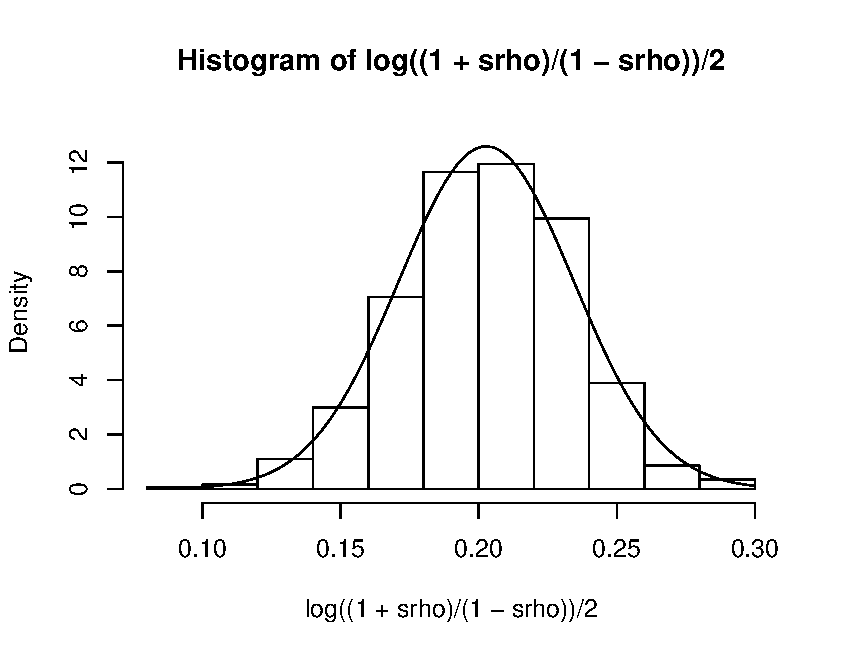
\includegraphics[scale=0.7]{pics/fisher_rho_hist}
%\end{center}	
%\end{frame}

%\begin{frame}[fragile]{}
%Fisher's z-transform test is implemented in \textsc{R} as \texttt{cor.test}.
%   \begin{lstlisting}
%> set.seed(1); n <- 100; rho <- 0.2
%> x <- mvrnorm(n,c(0,0),matrix(c(1,rho,rho,1),2,2))
%> cor.test(x[,1], x[,2], method = "pearson") 
%# Pearson's product-moment correlation
%data:  x[, 1] and x[, 2]
%t = 6.2913, df = 998, p-value = 4.704e-10
%alternative hypothesis: true correlation is not equal to 0
%95 percent confidence interval:
% 0.1349527 0.2542267
%sample estimates:
%      cor 
%0.1953118 
% \end{lstlisting}
%Try the same with $\rho=0$.\\[.2cm]
%\begin{beamercolorbox}[wd=\paperwidth,sep=5pt]{important}
%Non-gaussianity may invalidate the test and affect its power.	
%\end{beamercolorbox}
%\end{frame}

\begin{frame}[fragile,label=tau]{Basic nonparametric test}
\begin{block}{Kendall's tau test for non-Gaussian data}
Suppose a bivariate sample $(x_i,y_i)$ for $i=1,\ldots,n$ is given.\\[.2cm]
Pair $(x_i,y_i)$ , $(x_j,y_j)$ is \alert{concordant} if $(x_i,y_i)< (x_j,y_j)$ or $(x_i,y_i)> (x_j,y_j)$. Otherwise  \alert{discordant}.\\[.2cm]
Define $\tau_{XY}\;=\;\tfrac{(\#\mbox{concordant})-(\#\mbox{discordant})}{{n\choose 2}}\;\in\;  [-1,1]$.\\[.2cm]
Test based on Kendell's $\tau$ statistic is implemented in \textsc{R} as \texttt{cor.test}.
   \begin{lstlisting}
> set.seed(1); n <- 200; rho <- 0.2; Z <- runif(n); 
> X <- runif(n)^2+sqrt(rho)*Z; Y <- runif(n)+sqrt(rho)*Z
> cor.test(X, Y, method = "pearson")$p.value
[1] 0.03417231
> cor.test(X, Y, method = "kendall")$p.value
[1] 0.01100592
 \end{lstlisting}
\end{block}
\end{frame}


\begin{frame}[fragile]{Non-Gaussianity issue}
\begin{beamercolorbox}[wd=\paperwidth,sep=5pt]{important}
Vanishing covariance does not imply independence!
\end{beamercolorbox}
\begin{lstlisting}
# generate sample from two uncorrelated but dependent random variables
> set.seed(1); n <- 200
> A <- runif(n)-1/2; B <- runif(n)-1/2
> X <- t(c(cos(pi/4),-sin(pi/4)) %*% rbind(A,B))
> Y <- t(c(sin(pi/4),cos(pi/4)) %*% rbind(A,B))
> cor.test(X,Y, method = "pearson")
# Pearson's product-moment correlation
data:  X and Y
t = -0.84711, df = 198, p-value = 0.398
alternative hypothesis: true correlation is not equal to 0
95 percent confidence interval:
 -0.1971897  0.0793095
sample estimates:
        cor 
-0.06009275 \end{lstlisting}
$X$ and $Y$ are uncorrelated but dependent!
\end{frame}

\begin{frame}{}
\begin{center}
	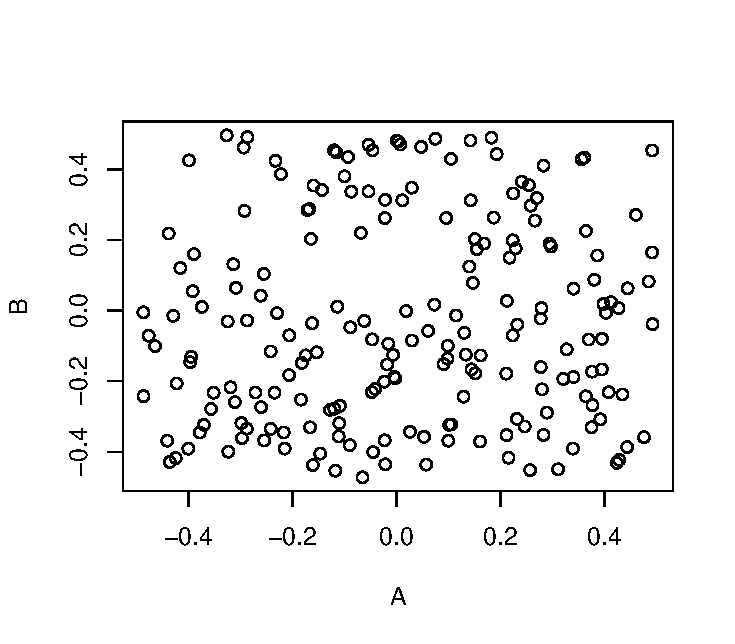
\includegraphics[width=0.5\textwidth]{pics/ABplot}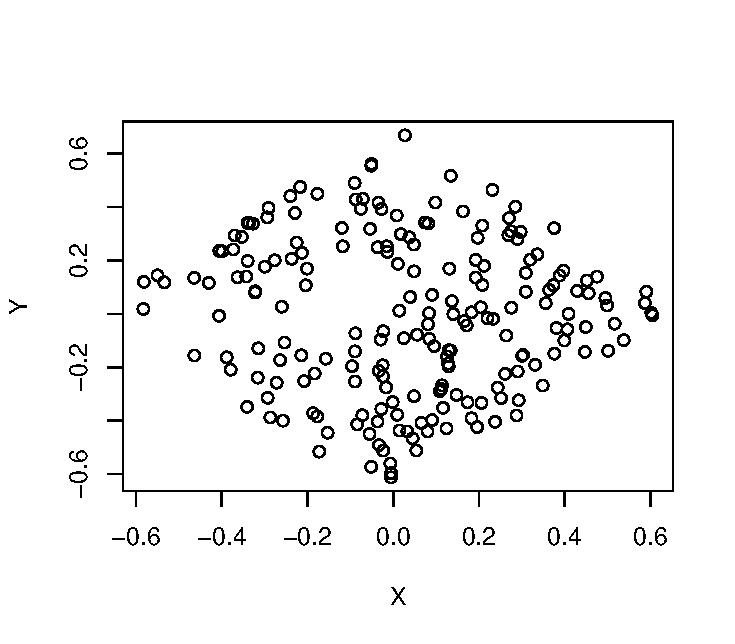
\includegraphics[width=0.5\textwidth]{pics/XYplot}	
\end{center}
	We see that $X$ and $Y$ are highly dependent. 
\end{frame}

\begin{frame}[fragile,label=zerocor]{Test based on distance correlation}
\alert{Distance correlation} $\mathcal R(X,Y)$ provides a test which applies when 
$X$, $Y$ are two random \textbf{vectors} of any dimensions.\\[.2cm]
$\mathcal R(X,Y)=0$ if and only if $X$ and $Y$ are independent.\\[.2cm]
The sample version of $\mathcal R(X,Y)$ gives a \alert{nonparametric} test of independence. \\[.2cm]
%This is also implemented in R in package \texttt{energy}.
\begin{lstlisting}
> library(energy); set.seed(1); n <- 200
> A <- runif(n)-1/2; B <- runif(n)-1/2
> X <- t(c(cos(pi/4),-sin(pi/4)) %*% rbind(A,B))
> Y <- t(c(sin(pi/4),cos(pi/4)) %*% rbind(A,B))
> dcor.test(X,Y,R=1000)

# dCor independence test (permutation test)
data:  index 1, replicates 1000
dCor = 0.21161, p-value = 0.004995
sample estimates:
      dCov       dCor    dVar(X)    dVar(Y) 
0.03999654 0.21160982 0.17870935 0.19990601 
\end{lstlisting}
Here $R=1000$ is the number of the permutation bootstrap replications.
\end{frame}

\begin{frame}[fragile]{Another cautionary example}
	Bowman\& Azzalini (1997) analyse aircraft wing span and speed data.	 \begin{center}
	 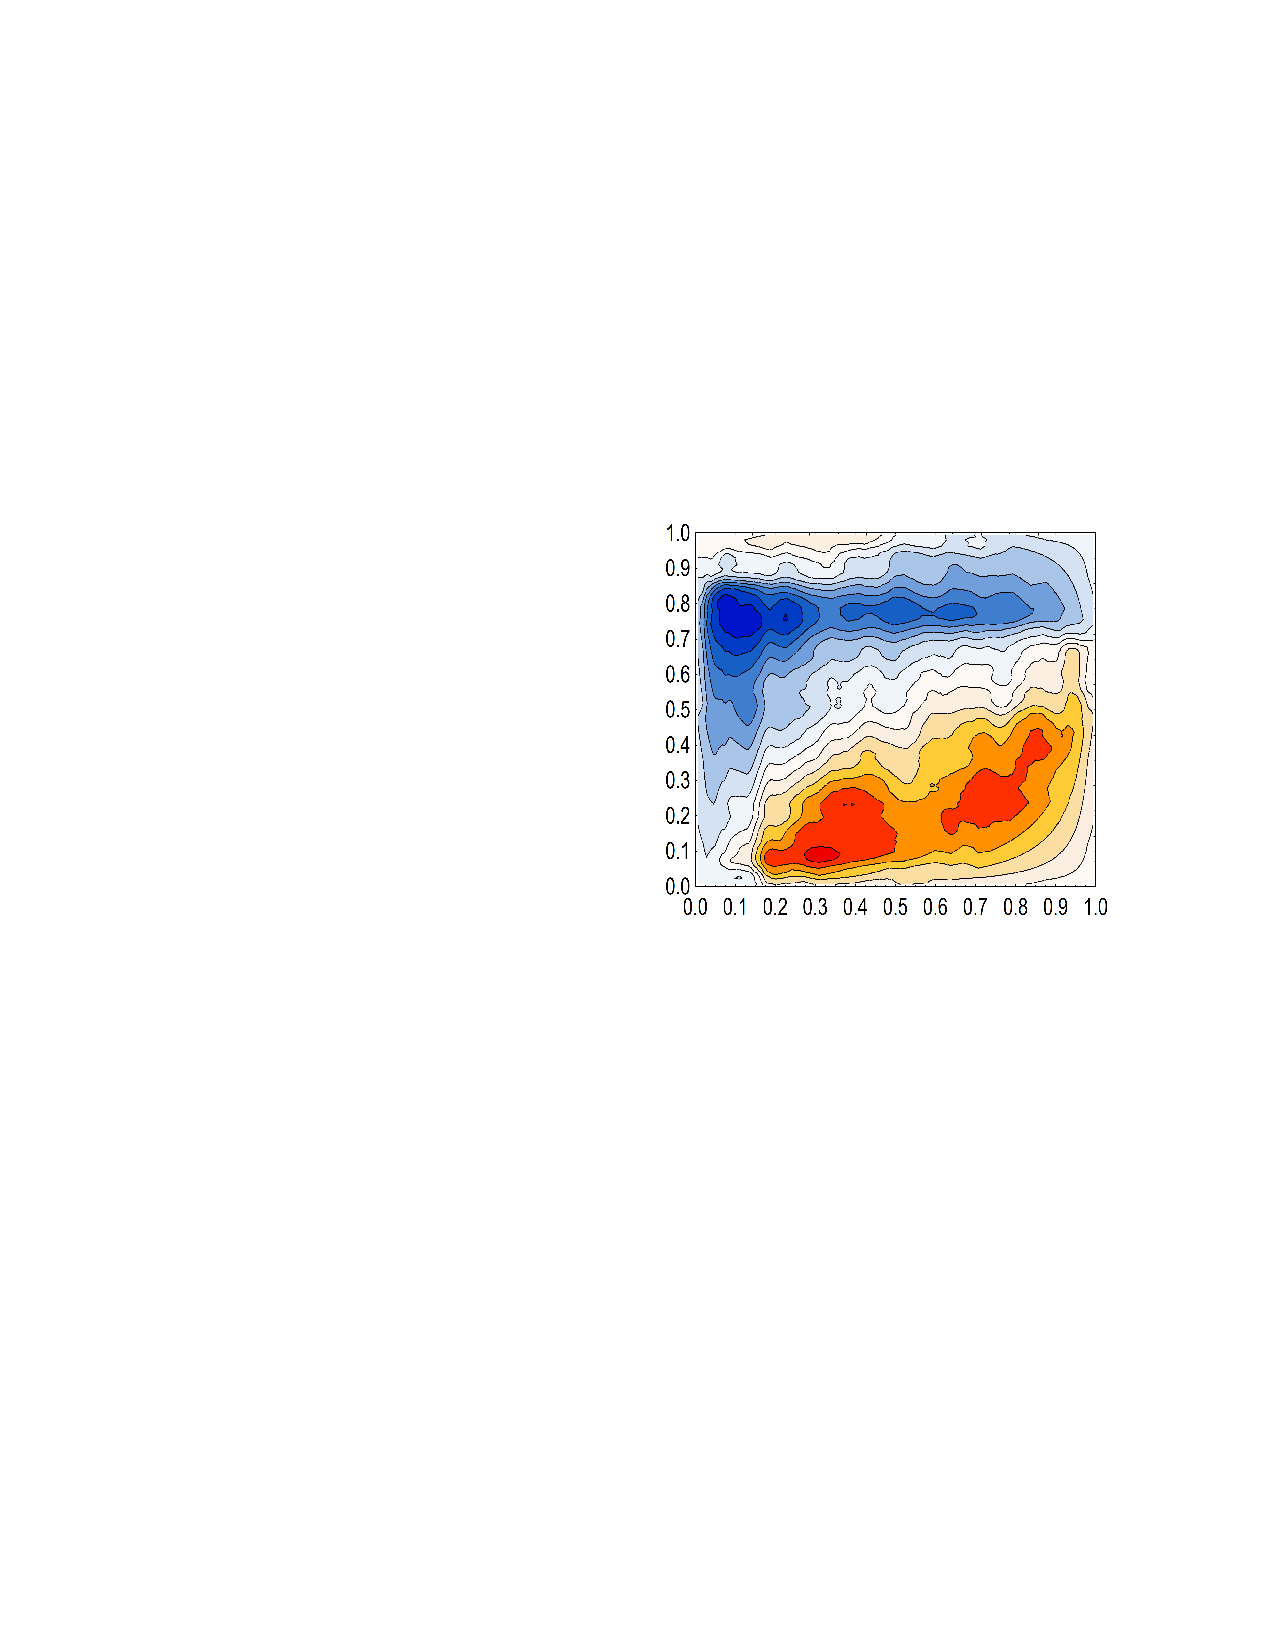
\includegraphics[scale=.5]{pics/aircraft}	 	
	 \end{center}
	 \begin{lstlisting}
> library(sm); set.seed(1); 
> X <- aircraft$Span
> Y <- aircraft$Speed
> cor.test(X,Y)$p.value
[1] 0.7816014
> dcor.test(X,Y,R=1000)$p.value
[1] 0.000999001
\end{lstlisting}
\end{frame}

\begin{frame}[fragile]{Tests for discrete data}
	\begin{alertblock}{$\chi^2$-test for discrete data}
   \begin{lstlisting}
> M <- as.table(rbind(c(762, 327, 468), c(484, 239, 477)))
> dimnames(M) <- list(gender = c("F", "M"),
+                     party = c("Democrat","Independent", "Republican"))

> (Xsq <- chisq.test(M))  # Prints test summary

Pearsons Chi-squared test

data:  M
X-squared = 30.07, df = 2, p-value = 2.954e-07
     
> Xsq$expected   # expected counts under the null
      party
gender Democrat Independent Republican
     F 703.6714    319.6453   533.6834
     M 542.3286    246.3547   411.3166
      \end{lstlisting}
\end{alertblock}
\texttt{df = 2} is the difference between $5$ (saturated model) and $3$ (independence)
\end{frame}



\begin{frame}[fragile]{Testing conditional independence}
Testing conditional independence is hard in general.\\[.2cm] 
For discrete data we have the asymptotic $\chi^2$-test.\\[.2cm]

Some parametric tests are implemented in the library \texttt{bnlearn}.\\
Many non-parametric methods have been implemented in \texttt{CondIndTest}
 \begin{lstlisting}
> library(CondIndTests); library(bnlearn); set.seed(1); n <- 100
> Z <- rnorm(n); X <- 4 + 2 * Z + rnorm(n); Y <- 3 * X^2 + Z + rnorm(n)
> CondIndTest(X,Y,Z, method = "KCI")$pvalue 
[1] 2.419926e-10
> bnlearn::ci.test(X,Y,Z)$p.value 
[1] 1.15458e-25
\end{lstlisting}
\medskip

{\scriptsize See Section 3 in: 
C. Heinze-Deml, J. Peters, N. Meinshausen, Invariant Causal Prediction for Nonlinear Models, Journal of Causal Inference, 2018.}
\bigskip

{\scriptsize See: \url{http://www.bnlearn.com/documentation/man/conditional.independence.tests.html}}
\end{frame}

\begin{frame}[label=SP]{Simpson's paradox: UC Berkeley admissions example}
		The admission figures of the grad school at UC Berkeley in 1973: 8442 (44\%) men, 4321 (35\%) women admitted.\\[.3cm] The same data conditioned on the department are:\\[.3cm]
\hspace{.7cm}\begin{tabular}{|c|c|c|c|c|}
\hline
\multirow{2}{*}{Department} & \multicolumn{2}{c|}{Men}   & \multicolumn{2}{c|}{Women} \\ \cline{2-5} 
                            & Applicants & Admitted       & Applicants & Admitted       \\ \hline
A                           & 825        & 62\%          & 108        & \textbf{82\%} \\ \hline
B                           & 560        & 63\%          & 25         & \textbf{68\%} \\ \hline
C                           & 325        & \textbf{37\%} & 593        & 34\%          \\ \hline
D                           & 417        & 33\%          & 375        & \textbf{35\%} \\ \hline
E                           & 191        & \textbf{28\%} & 393        & 24\%          \\ \hline
F                           & 373        & 6\%           & 341        & \textbf{7\%}  \\ \hline
\end{tabular}
\medskip

``Measuring bias is harder than is usually assumed, and the evidence is sometimes contrary to expectation.''\\[.3cm] \tiny(Bickel et al,  \textit{Sex Bias in Graduate Admissions: Data From Berkeley}, Science, 1975) 
\end{frame}

\begin{frame}[fragile]{}
	In R:
	\begin{lstlisting}
> library(gRim); data(UCBAdmissions)
> bnlearn::ci.test(x = "Gender" , y = "Admit", z = "Dept", test="x2",data = as.data.frame(UCBAdmissions))

Pearsons X^2
data:  Gender ~ Admit | Dept
x2 = 0, df = 6, p-value = 1
alternative hypothesis: true value is greater than 0

# gRim gives a slightly more refined output
> gRim::ciTest(as.data.frame(UCBAdmissions),set=~Gender+Admit+Dept)

set: [1] "Gender" "Admit"  "Dept"  
Testing Gender _|_ Admit | Dept 
Statistic (DEV):    0.000 df: 6 p-value: 1.0000 method: CHISQ

Slice information:
  statistic p.value df Dept
1         0       1  1    A
2         0       1  1    B
3         0       1  1    C
4         0       1  1    D
5         0       1  1    E
6         0       1  1    F
 \end{lstlisting}
% \includegraphics[scale=.3]{pics/UCB1} \includegraphics[scale=.3]{pics/UCB2}
\end{frame}



%
%\begin{frame}[fragile,label=SP2]{Florida murderers}
%Sentences in 4863 murder cases in Florida over the six
%years 1973-78
%\begin{center}
%\begin{tabular}{lcc} \hline
%&\multicolumn{2}{c}{Sentence}\\
%\cline{2-3}
%Murderer&Death&Other\\
%\hline Black&59&2547\\ White&72&2185\\
%\hline
%\end{tabular}
%\end{center}
%The table shows a greater proportion
% of white murderers receiving death sentence than black
%(3.2\% vs.\ 2.3\%).
%	\begin{lstlisting}
%> flor <- matrix(c(59,72,2547,2185),2,2)
%> dimnames(flor) <- list(Murderer=c("Black","White"),Sentence=c("Death","Other"))
%> chisq.test(flor)
%
%Pearsons Chi-squared test with Yates continuity correction
%data:  flor
%X-squared = 3.6117, df = 1, p-value = 0.05737
%\end{lstlisting}
%\end{frame}
%
%\begin{frame}[fragile]{Controlling for colour of victim}
%\begin{center}
%\begin{tabular}{llcc}
%\hline
%&&\multicolumn{2}{c}{Sentence}\\
%\cline{3-4}
%Victim&Murderer&Death&Other\\
%\hline
%Black&Black&11&2309\\
%&White&0&111\\
%White&Black&48&238\\
%&White&72&2074\\
%\hline
%\end{tabular}
%\end{center}
%Now the table for given colour
%of victim shows a very different picture.
%
%
%%\pause
%\smallskip
%
% In particular,
%note that 111 white murderers killed black victims and
%none were sentenced to death.
%	\begin{lstlisting}
%> flor <- c(11,48,0,72,2309,238,111,2074); dim(flor) <- c(2,2,2)
%> dimnames(flor) <- list(Victim=c("Black","White"),Murderer=c("Black","White"),Sentence=c("Death","Other"))
%> ciTest_table(flor,set=~Sentence+Murderer+Victim)
%Testing Sentence _|_ Murderer | Victim 
%Statistic (DEV):   67.980 df: 2 p-value: 0.0000 method: CHISQ
% \end{lstlisting}
%\end{frame}
%

\subsection{Multivariate normal distribution}
\begin{frame}[plain,noframenumbering]{}
\begin{center}
	{\huge \textcolor{DarkRed}{Conditional independence for Gaussian distributions}}
\end{center}
\end{frame}



\begin{frame}{Recall: Marginal and conditional distributions}
	Split $X$ into two blocks $X=(X_A,X_B)$. Denote $$\mu=(\mu_A,\mu_B)\qquad\mbox{and}\qquad\Sigma=\begin{bmatrix}
		\Sigma_{AA} & \Sigma_{AB}\\
		\Sigma_{BA} & \Sigma_{BB}
	\end{bmatrix}.$$
	\begin{block}{Marginal distribution}
		$X_A\sim N_{|A|}(\mu_A,\Sigma_{AA})$
	\end{block}
	\begin{block}{Conditional distribution}
		$X_A|X_B=x_B\sim N_{|A|}\left(\textcolor{red}{\small \mu_A+\Sigma_{AB}\Sigma_{BB}^{-1}(x_B-\mu_B)},\textcolor{blue}{\small \Sigma_{AA}-\Sigma_{AB}\Sigma_{BB}^{-1}\Sigma_{BA}}\right)$
		\begin{itemize}
			\item Note that the conditional covariance is constant.
		\end{itemize}
	\end{block}
%	\bigskip
%	\textbf{Example}: Consider a bivariate normal with $\mu=(0,2)$ and $\Sigma=\begin{bmatrix}
%		1 & 0.7\\0.7 & 1
%	\end{bmatrix}$. We have  $\E[X_1|X_2]={0.7}(X_2-2)$\; and\; ${\rm var}(X_1|X_2)=1-{0.7^2}= 0.51 $.
\end{frame}


\begin{frame}{Conditional independence}
\begin{alertblock}{Independence and conditional independence}
$X_i\indep X_j$ if and only if $\Sigma_{ij}=0$.\\[.3cm]
$X_i\indep X_j|X_{C}$\;\; if and only if \;\; $\Sigma_{ij}-\Sigma_{i,C}\Sigma_{C,C}^{-1}\Sigma_{C,j}=0$\\[.3cm]
Let $R=V\setminus \{i,j\}$. The following are equivalent:
\begin{itemize}
	\item $X_i\indep X_j|X_{R}$
	\item $\Sigma_{ij}-\Sigma_{i,R}\Sigma_{R,R}^{-1}\Sigma_{R,j}=0$
	\item \textcolor{blue}{$(\Sigma^{-1})_{ij}=0$}
\end{itemize}
\end{alertblock}
{\tiny Useful: \url{https://en.wikipedia.org/wiki/Block_matrix\#Block_matrix_inversion}}
%\begin{beamercolorbox}[wd=\paperwidth,sep=2pt]{notabene}	
%Central Limit Theorem provides the biggest motivation for Gaussian distributions.\end{beamercolorbox}
\end{frame}




\end{document}

